\documentclass[11pt,a4paper]{article}
\usepackage[margin=2.2cm]{geometry}
\usepackage{graphicx}
\usepackage{caption}
\usepackage{setspace}
\usepackage{float}
\graphicspath{{figures/}{_unused_not_cited/}}
\setstretch{1.15}
\setlength{\parindent}{0pt}
\setlength{\parskip}{0.35em}

\title{\textbf{Supplementary material}\\[0.4em]
\large Structure-informed CRISPR co-dependency maps the ARID1A-associated BAF
module across cancer cell lines}
\author{Zhiyong Tao, Juan Xiong, Yiwei Zhang, Chulin Zhong, Wenkai Gao, Guohua Fan}
\date{}

\begin{document}
\maketitle

\section*{Supplementary Figure S1}
\begin{figure}[H]
\centering
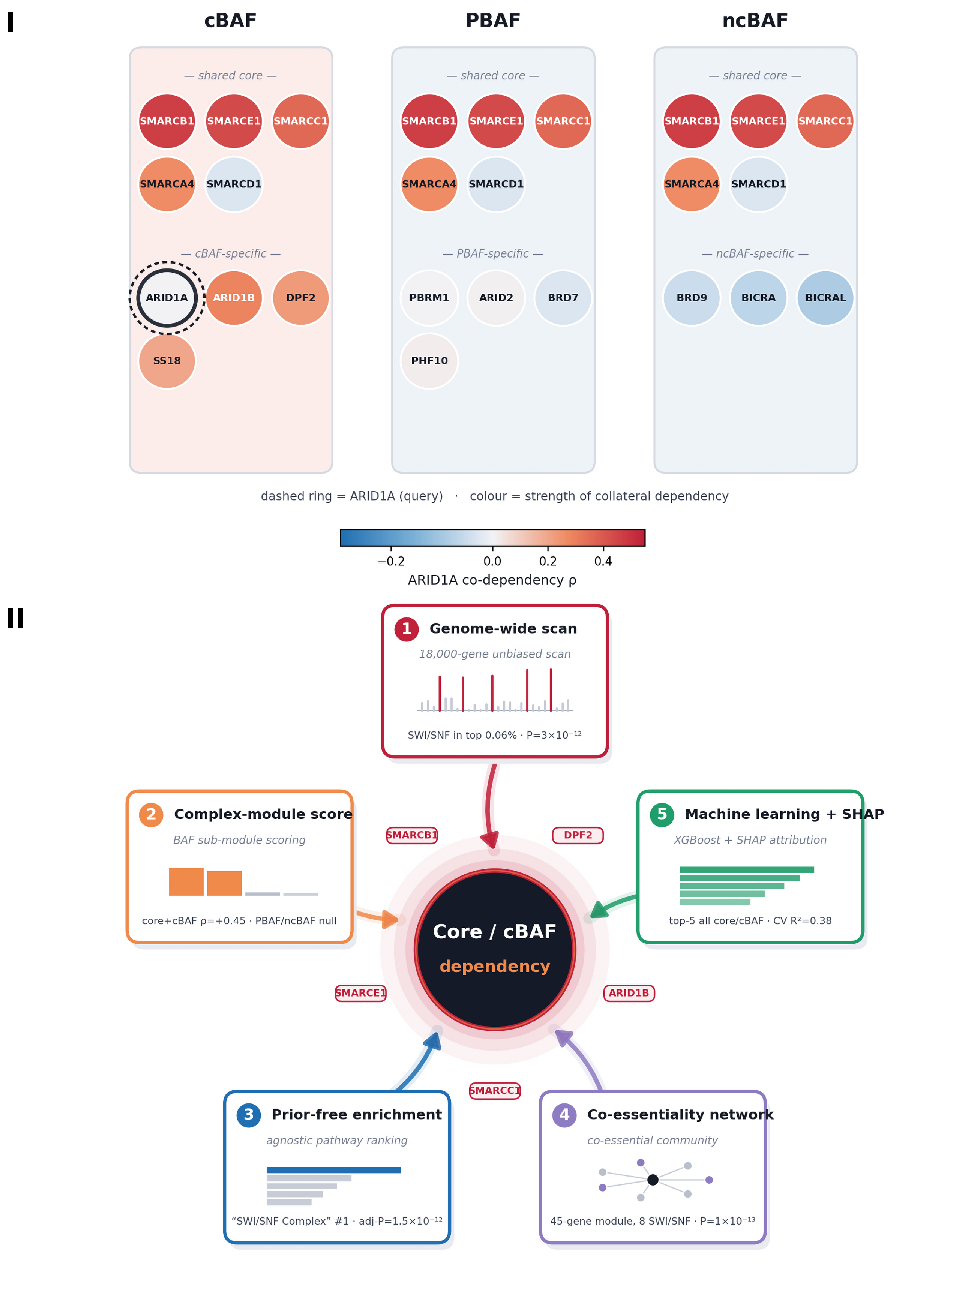
\includegraphics[width=0.94\textwidth]{FigS1_architecture.pdf}
\caption*{\textbf{Sub-complex composition and the structure of the convergence
argument.} (I) The three SWI/SNF sub-complexes drawn by subunit membership. Each
subunit is coloured by its pan-cancer co-dependency with ARID1A; ARID1A carries a
dashed ring. (II) The five methodologically distinct analyses and the subunits
each recovers. The analyses share one dependency matrix; four use no complex
composition during discovery.}
\end{figure}

\clearpage
\section*{Supplementary Figure S2}
\begin{figure}[H]
\centering
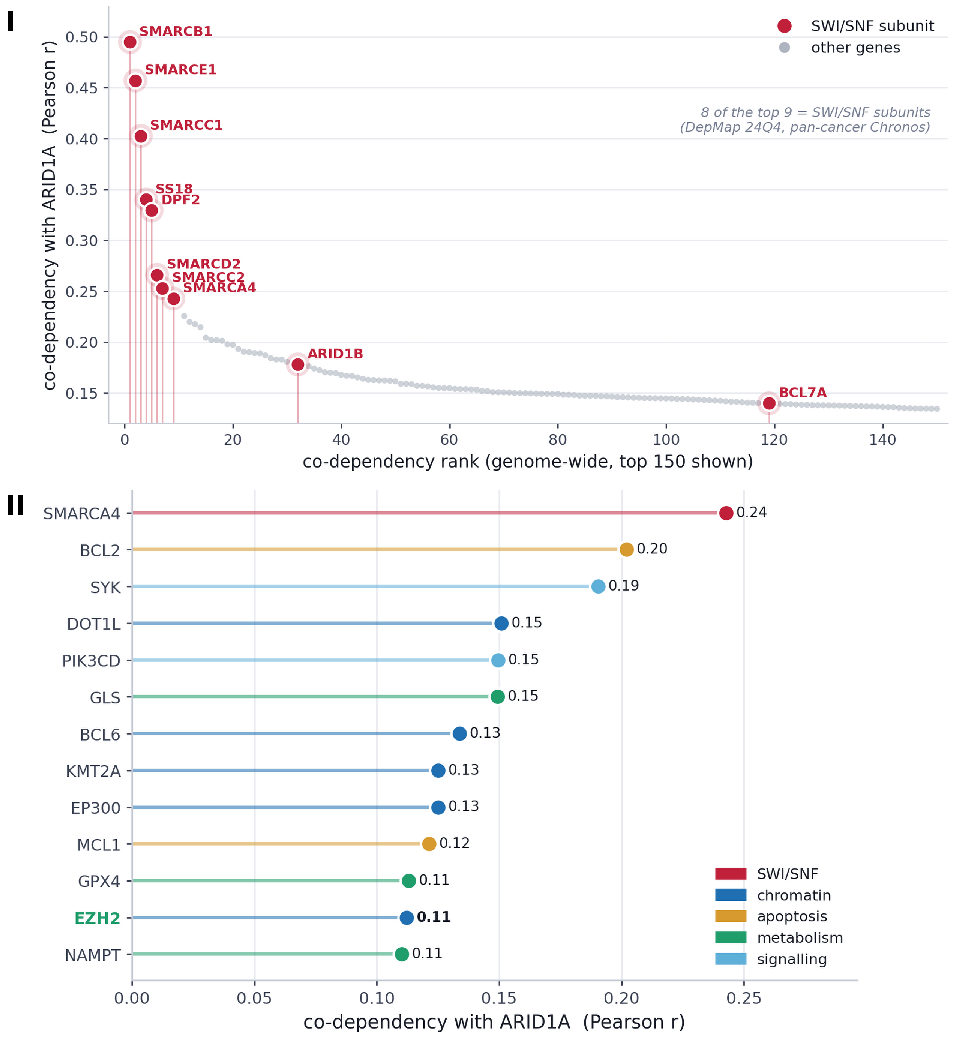
\includegraphics[width=0.98\textwidth]{FigS2_landscape.pdf}
\caption*{\textbf{Network-guided druggability prioritisation from the genome-wide
ARID1A co-dependency landscape.} (I) Top 150 genes ranked by pan-cancer
co-dependency in DepMap 24Q4. (II) Co-dependent genes for which a chemical probe
or clinical-stage inhibitor exists. This is a co-dependency-network overlay,
not a compound--target--pathway network-pharmacology analysis. The rankings
prioritise follow-up targets and do not establish genotype-selective efficacy.}
\end{figure}

\clearpage
\section*{Supplementary Figure S3}
\begin{figure}[H]
\centering
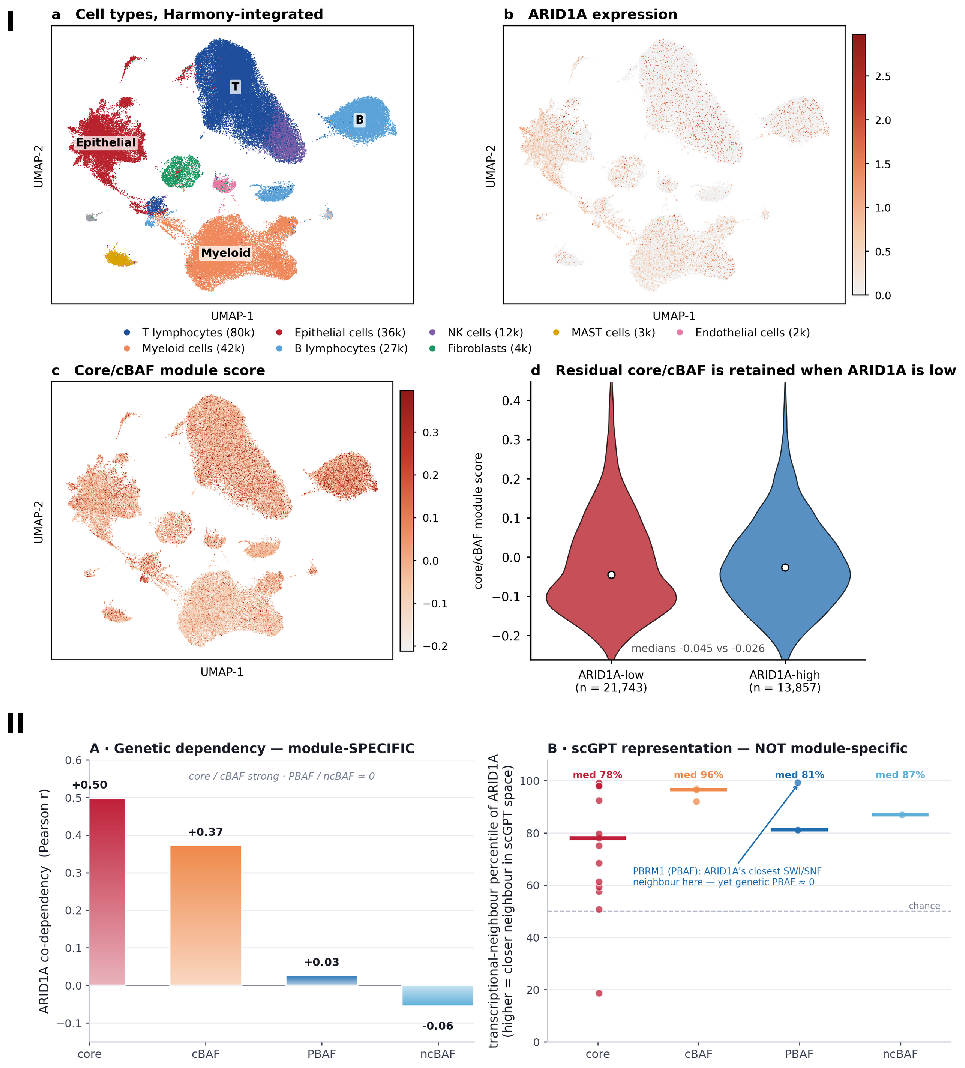
\includegraphics[width=0.98\textwidth]{FigM_singlecell.pdf}
\caption*{\textbf{Single-cell expression context and foundation-model control.}
(I) GSE131907 cell types, ARID1A expression, core/cBAF module score and the
descriptive cell-level split. Statistical inference in the main text uses 48
sample-level aggregates. (II) CRISPR co-dependency separates core/cBAF from
PBAF/ncBAF, whereas the scGPT transcriptional representation places every module
above chance and therefore does not resolve genetic specificity.}
\end{figure}

\clearpage
\section*{Supplementary Figure S4}
\begin{figure}[H]
\centering
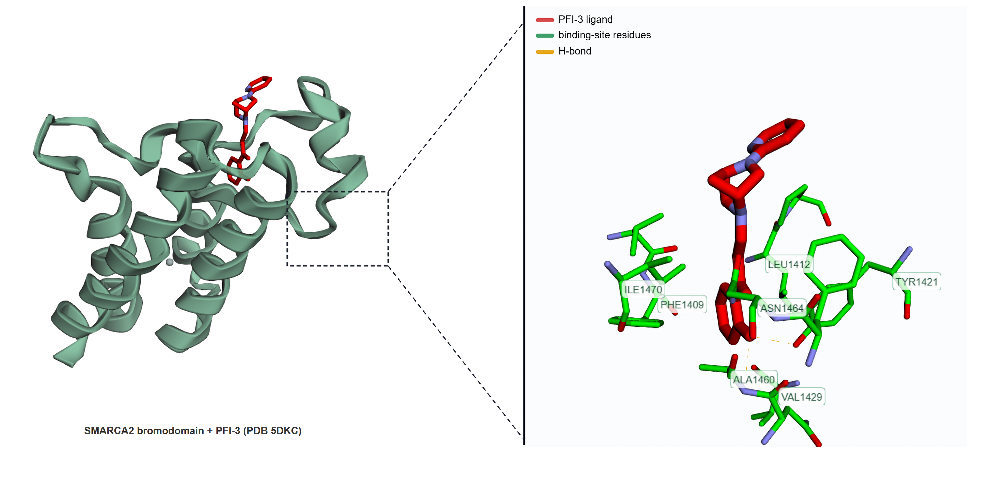
\includegraphics[width=0.92\textwidth]{Fig9_pose.pdf}
\caption*{\textbf{Crystallographic PFI-3 pose used as the docking positive
control.} Left, the SMARCA2/4 bromodomain co-crystal structure (PDB 5DKC) with
PFI-3 shown in red. Right, the binding-site close-up with contacting residues
labelled and the interaction with ASN1464 indicated. AutoDock Vina redocking
reproduced the deposited ligand pose at 0.48\,\AA{} heavy-atom RMSD. This panel
validates recovery of one known pose under the protocol; it does not validate
the FHD-286 blind-docking pose or establish genotype-selective activity.}
\end{figure}

\clearpage
\section*{Supplementary Figure S5}
\begin{figure}[H]
\centering
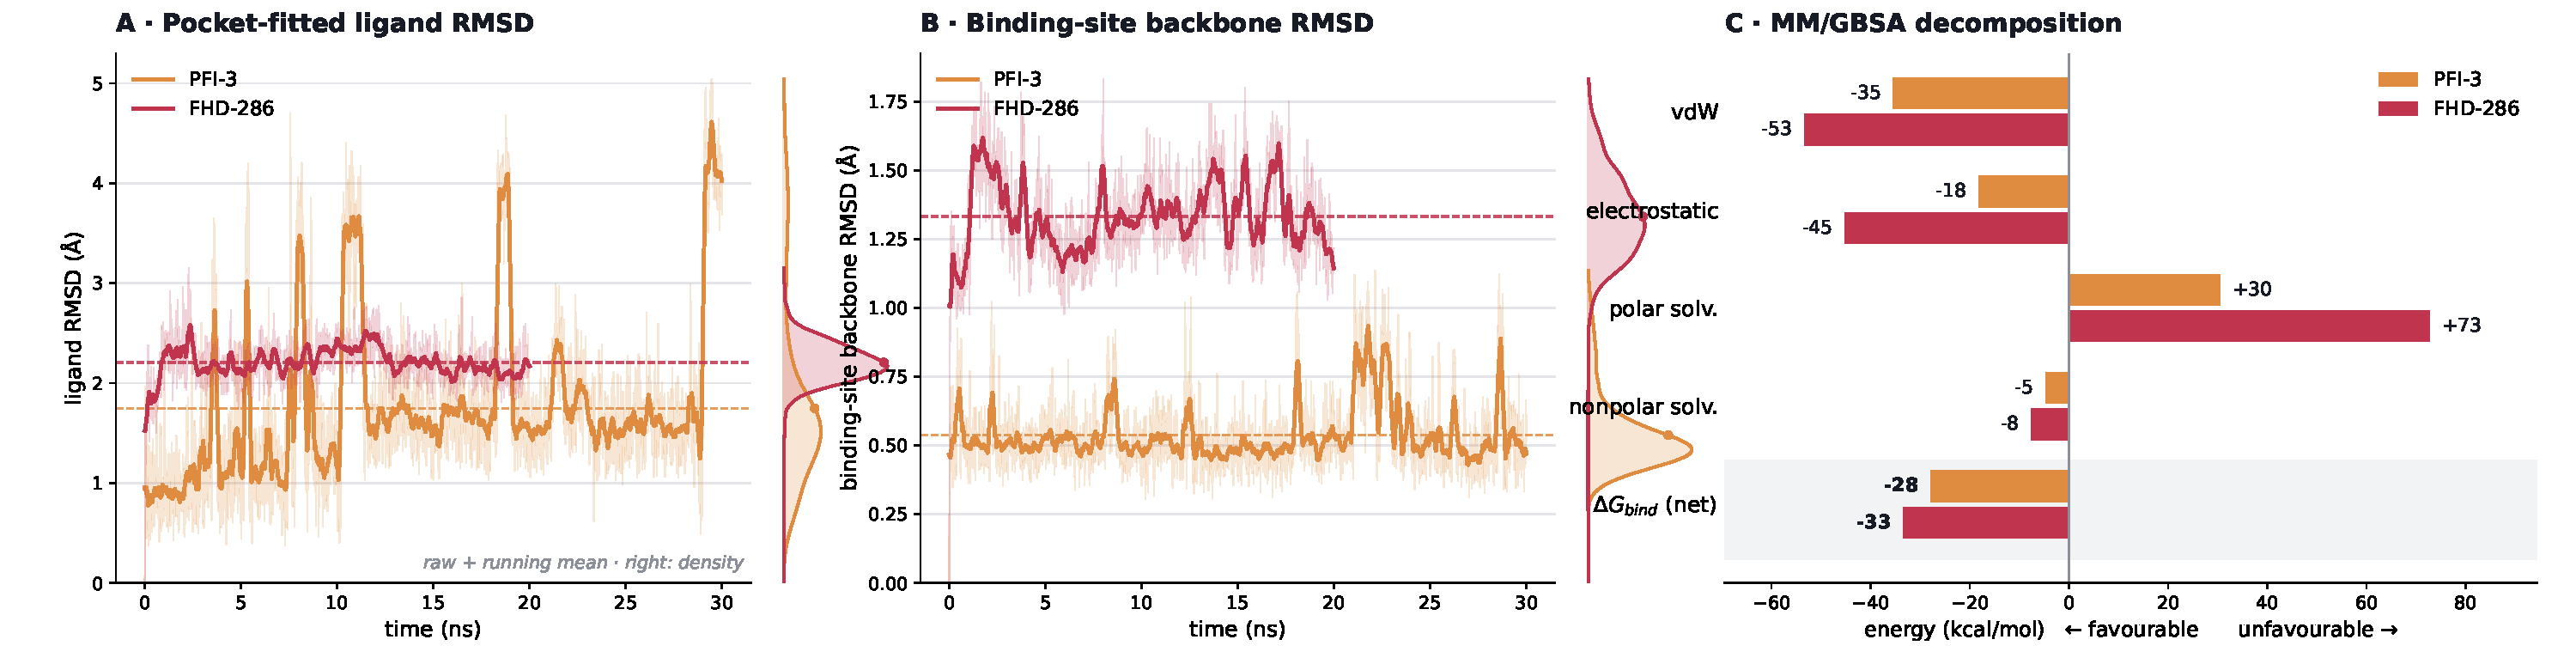
\includegraphics[width=\textwidth]{FigS5_md_verified20ns.pdf}
\caption*{\textbf{Single-trajectory molecular-dynamics checks of modelled
SWI/SNF ligand poses.} (\textbf{A}) Ligand RMSD after fitting the binding-site
residues, shown as raw frames, running means and framewise distributions.
(\textbf{B}) Binding-site backbone RMSD. PFI-3 was followed for 30\,ns from its
5DKC crystallographic pose; FHD-286 was followed for 20\,ns from the blind-docked
7VDT pose. (\textbf{C}) Single-trajectory MM/GBSA energy decomposition. The
reported means and standard deviations describe frames within one trajectory
per complex and are not uncertainty across independent simulations. These
calculations assess bounded pose behaviour over the sampled windows; they do not
validate the FHD-286 pose, provide absolute binding affinities or establish
ARID1A-genotype selectivity.}
\end{figure}

\clearpage
\section*{Supplementary Figure S6}
\begin{figure}[H]
\centering
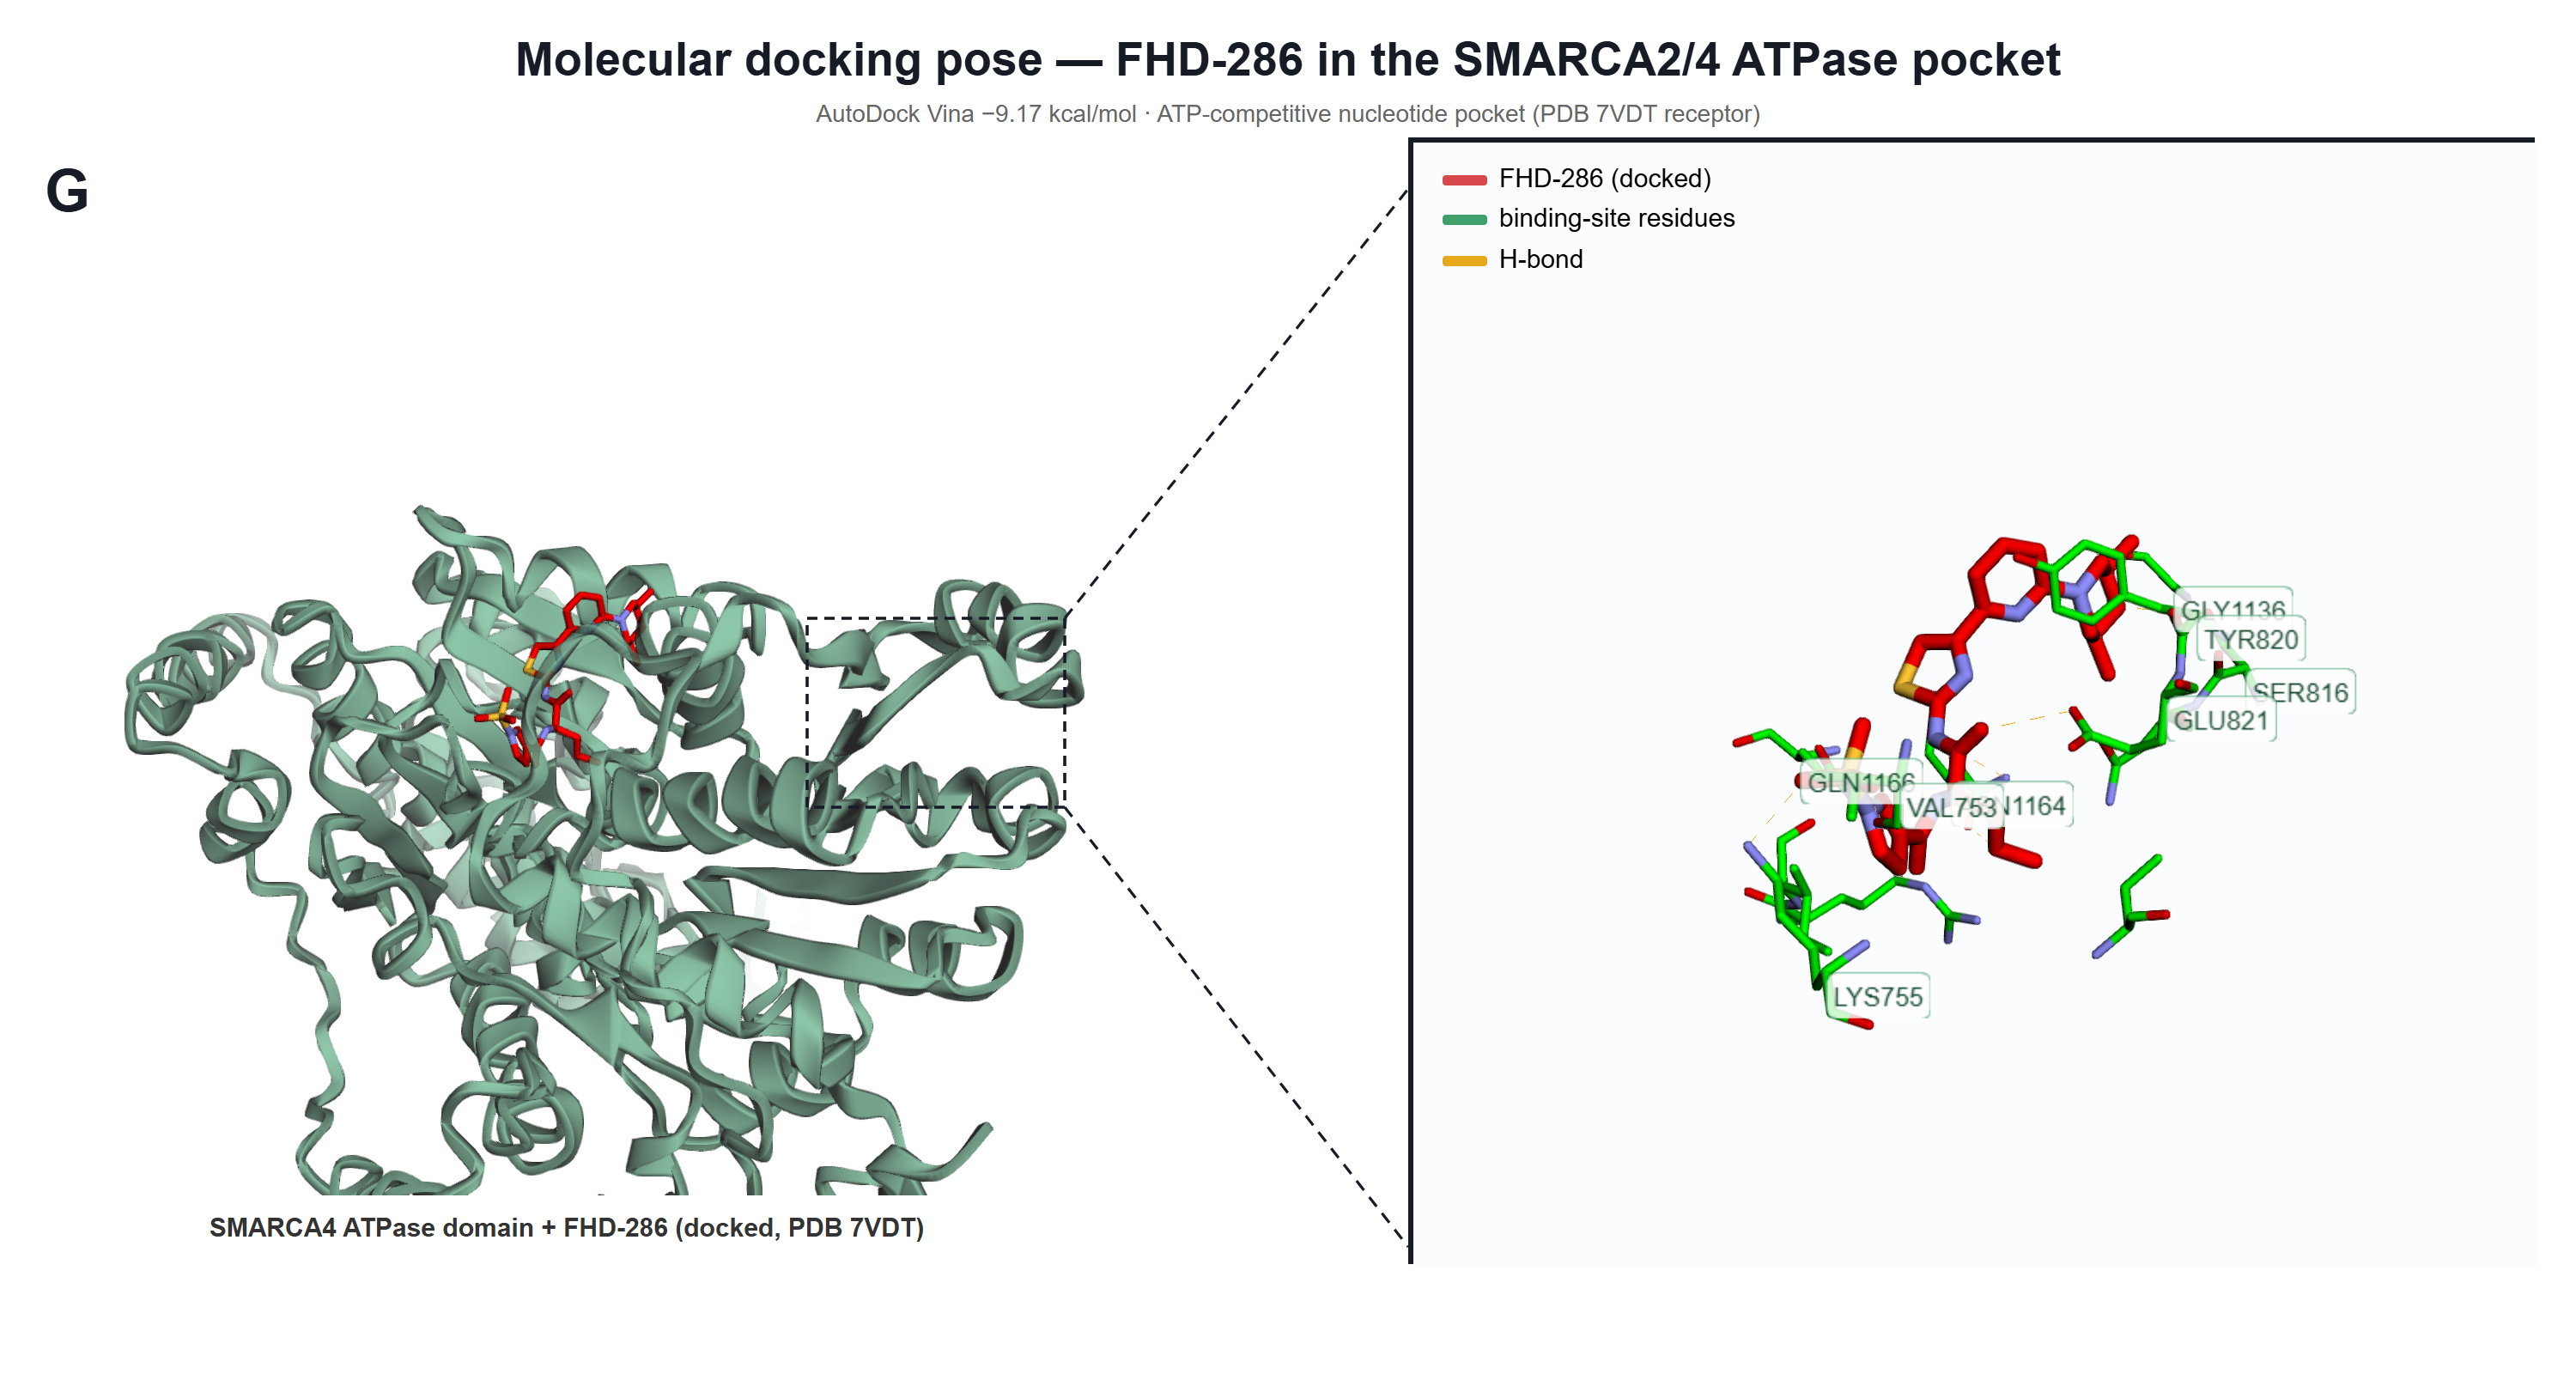
\includegraphics[width=\textwidth,trim=100bp 0 0 0,clip]{FigS6_fhd286_pose.png}
\caption*{\textbf{Blind-docked FHD-286 pose in the SMARCA4 ATPase nucleotide
pocket.} Whole-domain and close-up views show the modelled FHD-286 pose and
nearby pocket residues in PDB 7VDT; the AutoDock Vina score was
$-9.17$\,kcal\,mol$^{-1}$. Unlike the crystallographic PFI-3 positive control in
Supplementary Figure~S4, no public co-crystal validates this pose. Residue labels
therefore describe the modelled geometry and not experimentally established
contacts, affinity or ARID1A-genotype selectivity.}
\end{figure}

\clearpage
\section*{Supplementary Figure S7}
\begin{figure}[H]
\centering
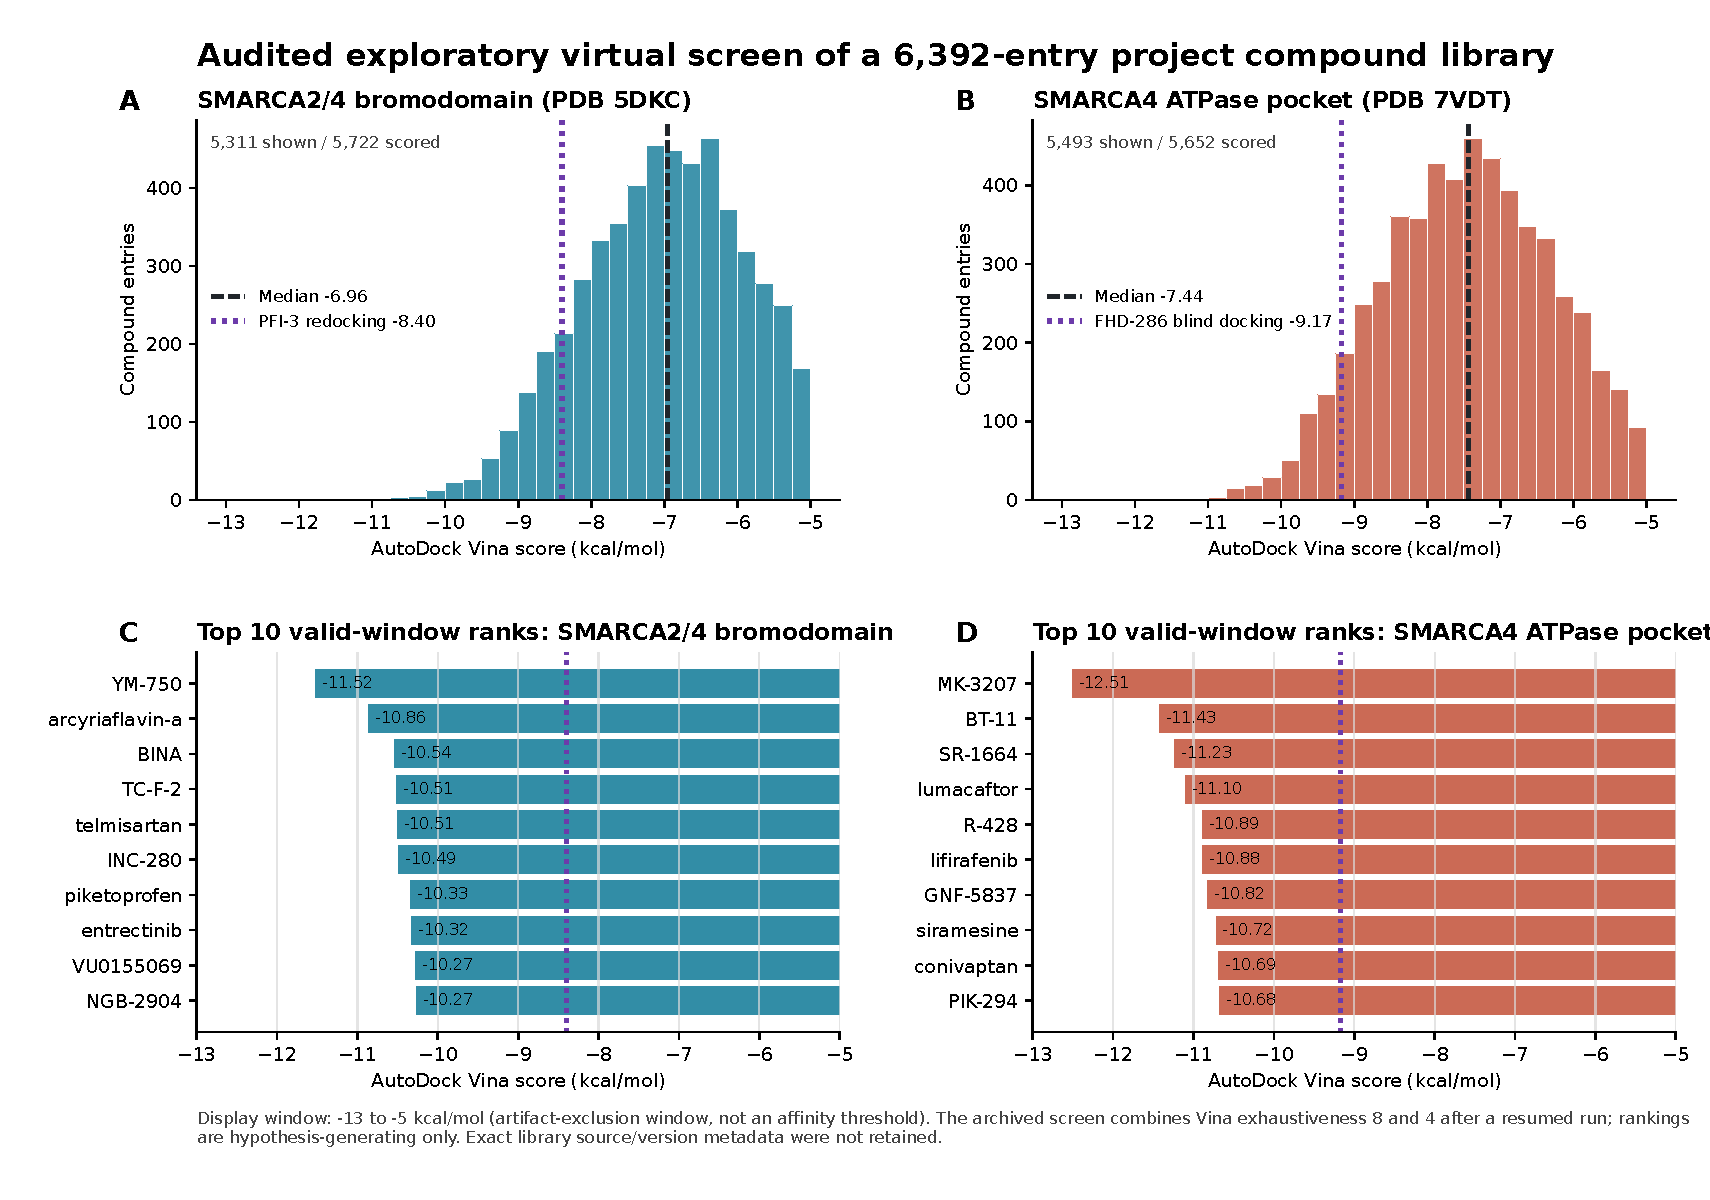
\includegraphics[width=\textwidth]{FigS7_virtual_screen_audited.pdf}
\caption*{\textbf{Audited exploratory virtual screen against the two modelled
SWI/SNF pockets.} (\textbf{A}, \textbf{B}) Score distributions for the SMARCA2/4
bromodomain (PDB 5DKC) and SMARCA4 ATPase pocket (PDB 7VDT), respectively;
dotted lines mark the PFI-3 and FHD-286 reference docking scores. Of 6{,}392
library entries, 5{,}722 and 5{,}652 returned numeric scores, of which 5{,}311
and 5{,}493 fell inside the project's $-13$ to $-5$\,kcal\,mol$^{-1}$
artefact-exclusion window. (\textbf{C}, \textbf{D}) Ten lowest scores in that
window for each pocket after collapsing duplicate identifiers to their lowest
score. The archived table combines an initial Vina run at exhaustiveness 8 and a
resumed run at exhaustiveness 4; exact library source/version metadata were not
retained. The display window is not an affinity threshold, and the rankings are
hypothesis-generating rather than evidence of binding or repurposing readiness.}
\end{figure}

\clearpage
\section*{Supplementary Figure S8}
\begin{figure}[H]
\centering
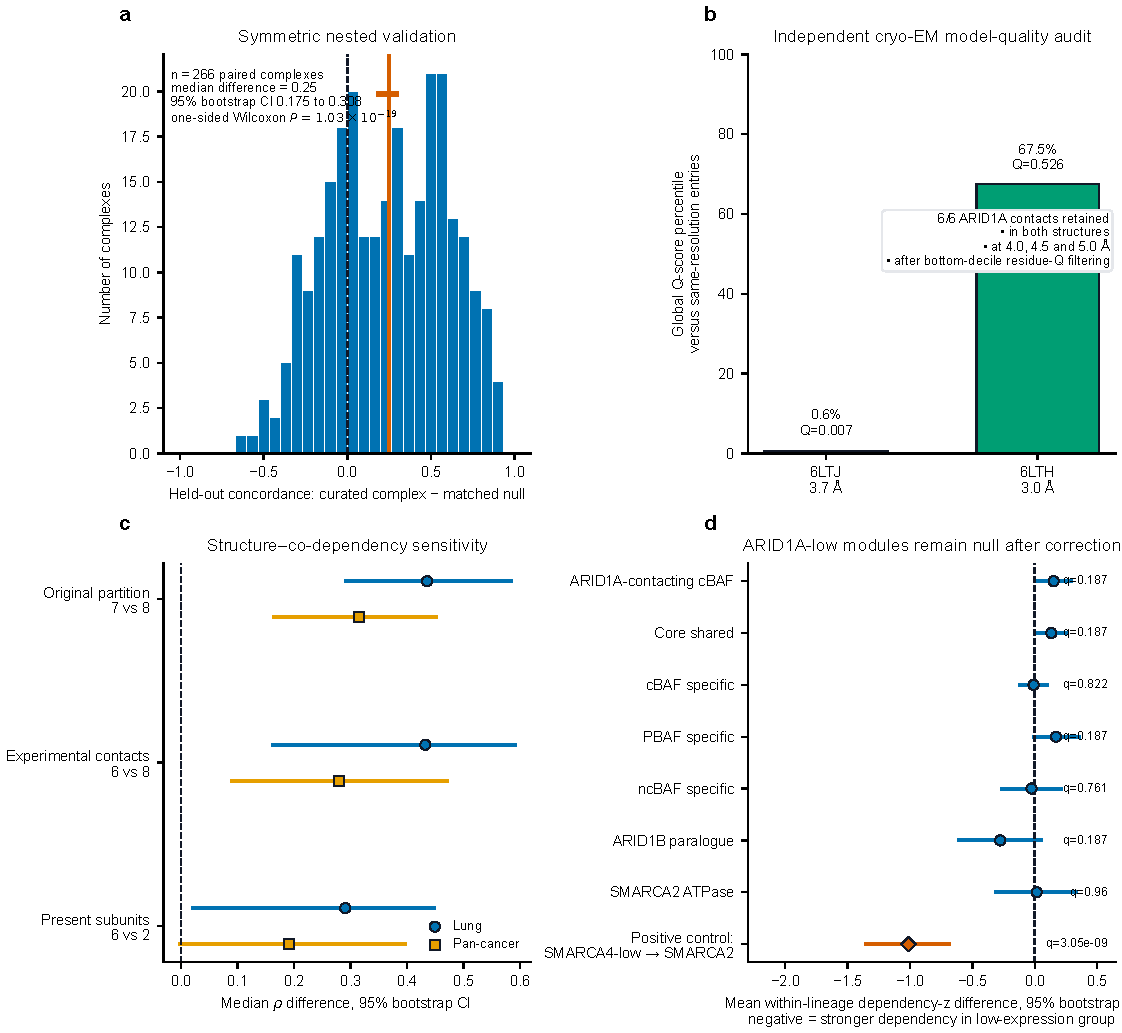
\includegraphics[width=0.92\textwidth]{FigS8_robustness_validation.pdf}
\caption*{\textbf{Robustness analyses for nested module refinement, structural
contact and conditional dependency.} (\textbf{a}) For 266 curated complexes,
the histogram shows the paired difference in held-out drop-identity concordance
between each real complex and its size-matched null modules. Anchor and dropped
member were selected only in the discovery half in both arms, then evaluated
unchanged in the validation half over 30 splits. The orange line is the paired
median difference (0.25) and the horizontal orange segment its 95\% percentile
bootstrap interval (0.175--0.308); the dashed line marks zero.
(\textbf{b}) wwPDB global Q-score percentiles relative to entries at the same
resolution. The full 6LTJ model is low quality globally, whereas the independent
6LTH base-module deposit is above the median; nevertheless, all six binary
ARID1A contact calls persist in both deposits, across 4.0--5.0\,\AA{} cutoffs and
after bottom-decile residue-Q filtering. (\textbf{c}) Median co-dependency
difference between contacting and non-contacting groups under three structural
definitions, with 95\% bootstrap intervals. Lung and pan-cancer estimates are
shown separately; exact two-sided Mann--Whitney tests are significant for the
original 7-vs-8 and experimental-contact-only 6-vs-8 definitions
($P\leq0.0127$), whereas the 6-vs-2 restriction is underpowered ($P=0.286$).
(\textbf{d}) Mean within-lineage dependency-$z$ difference for the bottom 10\%
of ARID1A protein abundance versus the remainder, with 95\% bootstrap intervals
and BH-adjusted $q$ values (52 low and 483 remaining lines). No module passes
correction. The prespecified pipeline control applies the same design to the
bottom 10\% of SMARCA4 mRNA and detects stronger SMARCA2 dependency (102 low
lines; $\Delta z=-1.012$, 95\% interval $-1.355$ to $-0.689$;
$q=3.05\times10^{-9}$). Intervals use 20{,}000 bootstrap resamples with seed
20260901.}
\end{figure}

\end{document}
